The \nameref{ch:problem} mainly described the needs which the Flashmap System might be able to accomodate, and on page~\pageref{sec:intro_flashmap} generic features of such a system is described. Although the term Flashmap System is intended for describing any system including these features, when having to evaluate the idea one has to evaluate one or multiple specific implementations of that idea. Therefore this part will specify the design features of the specific tool developed within this project, along with arguments in favour of and against these choices and their considerations, and the process with which they are incorporated within the tool itself. This description will follow the different steps of the Generic Model \cite{genericmodel}, which is displayed in figure~\ref{fig:genericmodel}.

\begin{figure}[h]
    \centering
    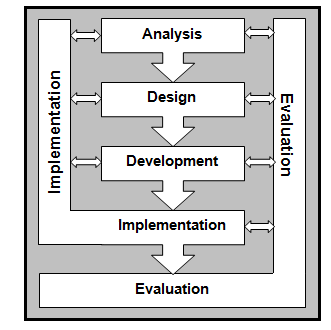
\includegraphics[width=0.5\textwidth]{img/genericmodel}
    \caption{The generic model by \protect\citeA{genericmodel}\label{fig:genericmodel}}
\end{figure}

The first step consists of analysing the context, learner and task characteristics in order derive their possibilities and requirements. Based on these together with general design guidelines provided by educational literature, design choices can be made and argued for within the next step. When these choices have been made, they can be developed and incorporated within the product. When the product then is finished it can be implemented within the context and evaluated. As can be seen in the model, the implementation and evaluation play an important part throughout the design process, rather than them being seperate steps at the end, and will therefore already be addressed during the description of the first three steps. Furthermore, these seperate steps will be described in the next part, which describes the research conducted within this project. Finally, rather than addressing the design and development in seperate chapters, they will be described alongside each other within the chapters describing the separate facets of the product. INSERT SEPARATE FACETS OF THE PRODUCT
